\section{Introduction}
\label{sec:introduction}

% preface

Variational inference is a computationally efficient approach for
approximating posterior distributions. The idea is to specify a
tractable family of distributions of the latent variables and then to
minimize the Kullback-Leibler divergence  from it to the posterior. Combined
with stochastic optimization, variational inference can scale complex
statistical models to massive data sets~\citep{hoffman2013stochastic,toulis2014implicit,tran2015stochastic}.

Both the computational complexity and accuracy of variational
inference are controlled by the factorization of the variational
family. To keep optimization tractable, most algorithms use the
fully-factorized family, also known as the mean-field family, where each
latent variable is assumed independent. Less common, structured
mean-field methods slightly relax this assumption by preserving some
of the original structure among the latent
variables~\citep{saul1995exploiting}. Factorized distributions enable
efficient variational inference but they sacrifice accuracy. In the
exact posterior, many latent variables are dependent and mean-field
methods, by construction, fail to capture this dependency.

% our procedure

To this end, we develop \gls{CVI}.
\Gls{CVI} augments the traditional variational distribution with a
copula, which is a flexible construction for learning dependencies in
factorized distributions~\citep{frechet1960tableaux}.  This strategy has many advantages over
traditional \glsunset{VI}\gls{VI}: it reduces bias; it is less sensitive to local optima;
it is less sensitive to hyperparameters; and it helps characterize and
interpret the dependency among the latent variables.  Variational
inference has previously been restricted to either generic inference
on simple models---where dependency does not make a significant
difference---or writing model-specific variational updates. \Gls{CVI}
widens its applicability, providing generic inference that finds
meaningful dependencies between latent variables.


In more detail, our contributions are the following.

\textbf{A generalization of the original procedure in variational
  inference}. \Gls{CVI} generalizes variational inference for
mean-field and structured factorizations: traditional
\glsunset{VI}\gls{VI} corresponds
to running only one step of our method. It uses coordinate descent,
which monotonically decreases the KL divergence to the posterior by
alternating between fitting the mean-field parameters and the copula
parameters. Figure \ref{fig:gaussian} illustrates \gls{CVI} on a toy
example of fitting a bivariate Gaussian.

\textbf{Improving generic inference}.  \Gls{CVI} can be applied to any
inference procedure that currently uses the mean-field or structured
approach.  Further, because it does not require specific knowledge of
the model, it falls into the framework of black box variational
inference~\citep{ranganath2014black}.  An investigator need only write
down a function to evaluate the model log-likelihood. The rest of the
algorithm's calculations, such as sampling and evaluating gradients, can be placed in a library.

\textbf{Richer variational approximations}.  In experiments, we demonstrate
\gls{CVI} on the standard example of Gaussian mixture models.  We
found it consistently estimates the parameters, reduces sensitivity to
local optima, and reduces sensitivity to hyperparameters. We also
examine how well \gls{CVI} captures dependencies on the latent space
model~\citep{hoff2001latent}. \Gls{CVI} outperforms competing methods
and significantly improves upon the mean-field approximation.

\begin{figure}[t]
\begin{minipage}{\textwidth}
  \begin{minipage}[b]{0.245\textwidth}
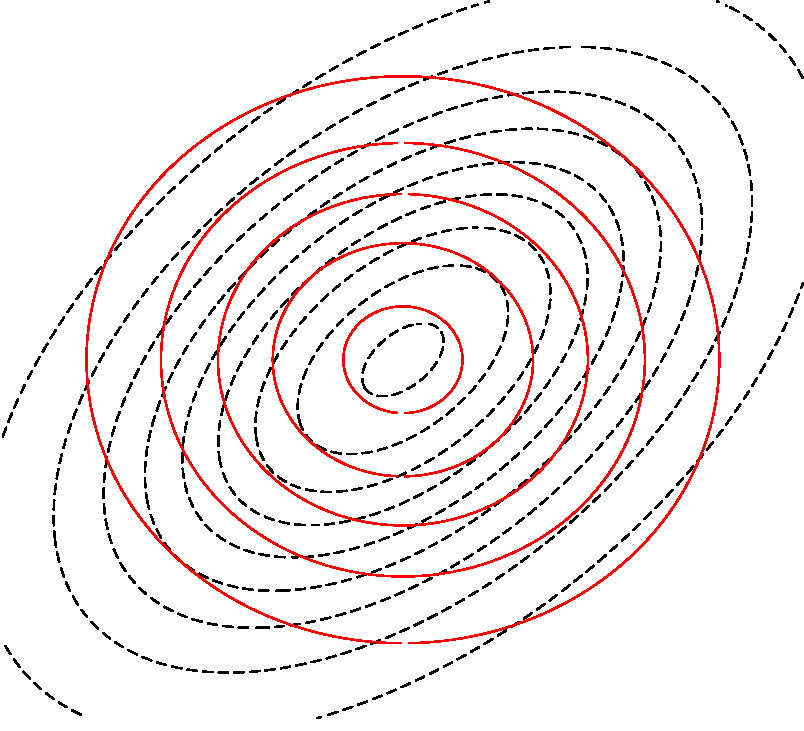
\includegraphics[width=\textwidth]{img/bivariate_gaussian_1.pdf}
  \end{minipage}
  \hfill
  \begin{minipage}[b]{0.245\textwidth}
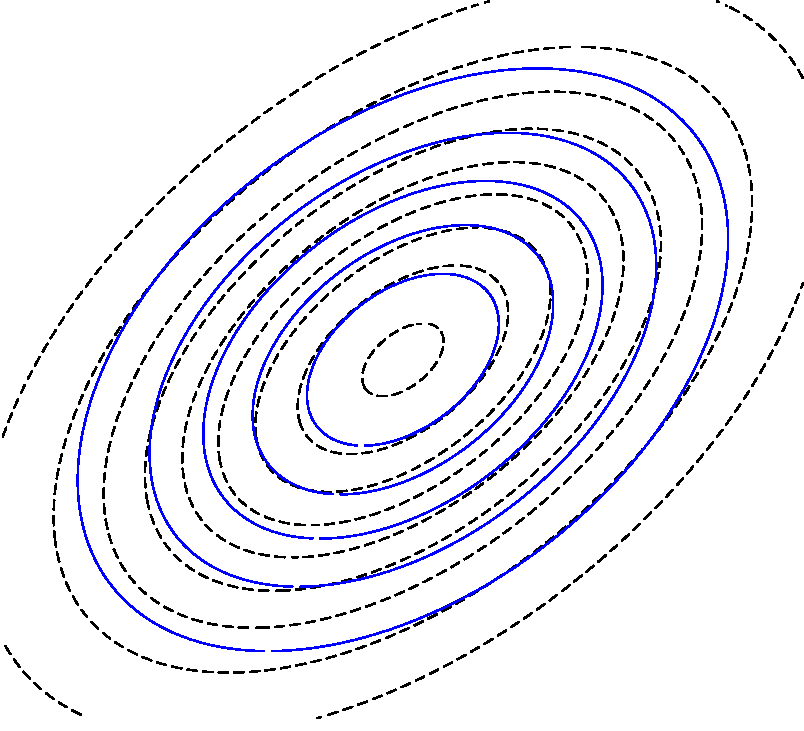
\includegraphics[width=\textwidth]{img/bivariate_gaussian_2.pdf}
  \end{minipage}
  \hfill
  \begin{minipage}[b]{0.245\textwidth}
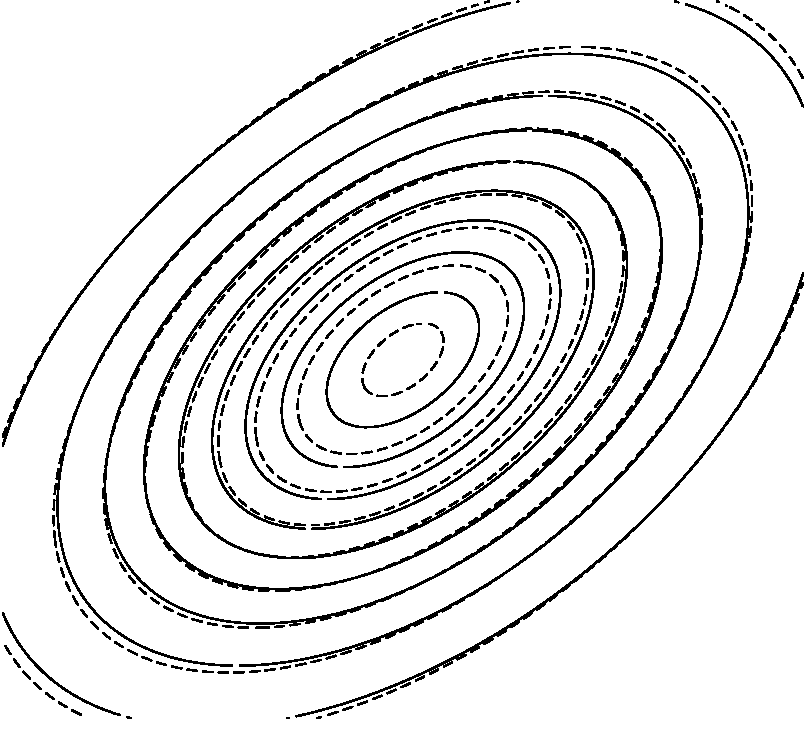
\includegraphics[width=\textwidth]{img/bivariate_gaussian_3.pdf}
  \end{minipage}
  \hfill
  \begin{minipage}[b]{0.245\textwidth}
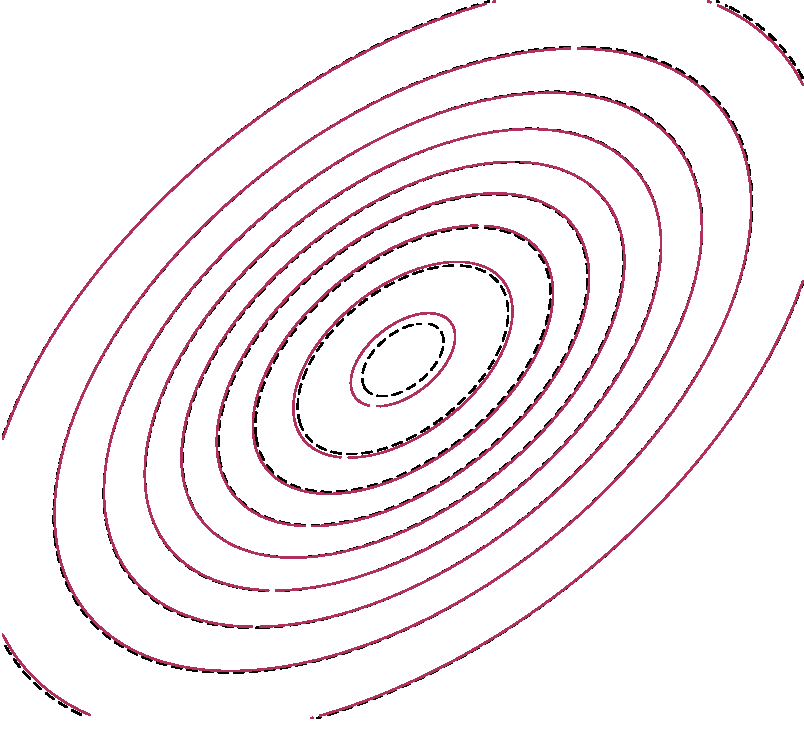
\includegraphics[width=\textwidth]{img/bivariate_gaussian_4.pdf}
  \end{minipage}
\end{minipage}
\caption{\label{fig:gaussian}Approximations to an
elliptical Gaussian. The mean-field (\textcolor{purple}{red}) is
restricted to fitting independent one-dimensional Gaussians, which is the first
step in our algorithm. The second step (\blue{blue}) fits a copula which models
the dependency. More iterations alternate: the third refits the mean-field
(\green{green}) and the fourth refits the copula
(\red{cyan}),
demonstrating convergence to the true posterior.}
\end{figure}


%%% Local Variables:
%%% mode: latex
%%% TeX-master: "nips2015"
%%% End:
